% ====================================================================
% LAMPIRAN (APPENDICES)
% ====================================================================
% File ini berisi lampiran penelitian.
% Lampiran dapat mencakup:
% - Data mentah
% - Kode sumber (untuk research komputasi)
% - Tabel detail/besar
% - Instrumen penelitian (kuesioner, interview guide)
% - Dokumen pendukung lainnya
%
% EDIT konten sesuai dengan lampiran penelitian Anda.
% ====================================================================

\appendix
\frontmatterchapter{LAMPIRAN}
\noindent\textbf{Lampiran - Alur Implementasi Sistem}

\begin{figure}[H]
\centering
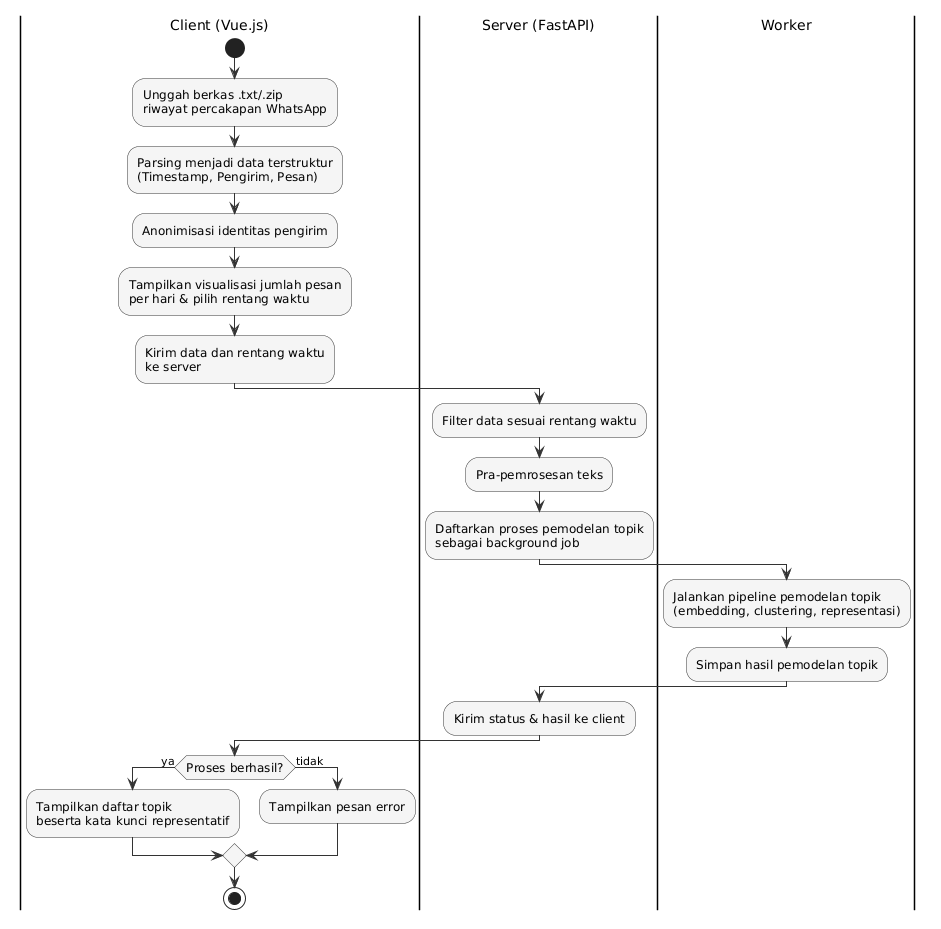
\includegraphics[width=0.9\textwidth]{images/bab-3-alur-implementasi-sistem.png}
\caption{Alur Implementasi Sistem}
\label{fig:bab-3-alur-implementasi-sistem}
\end{figure}

\newpage
\noindent\textbf{Lampiran - Alur Teknis Implementasi Sistem Web}

\begin{figure}[H]
\centering
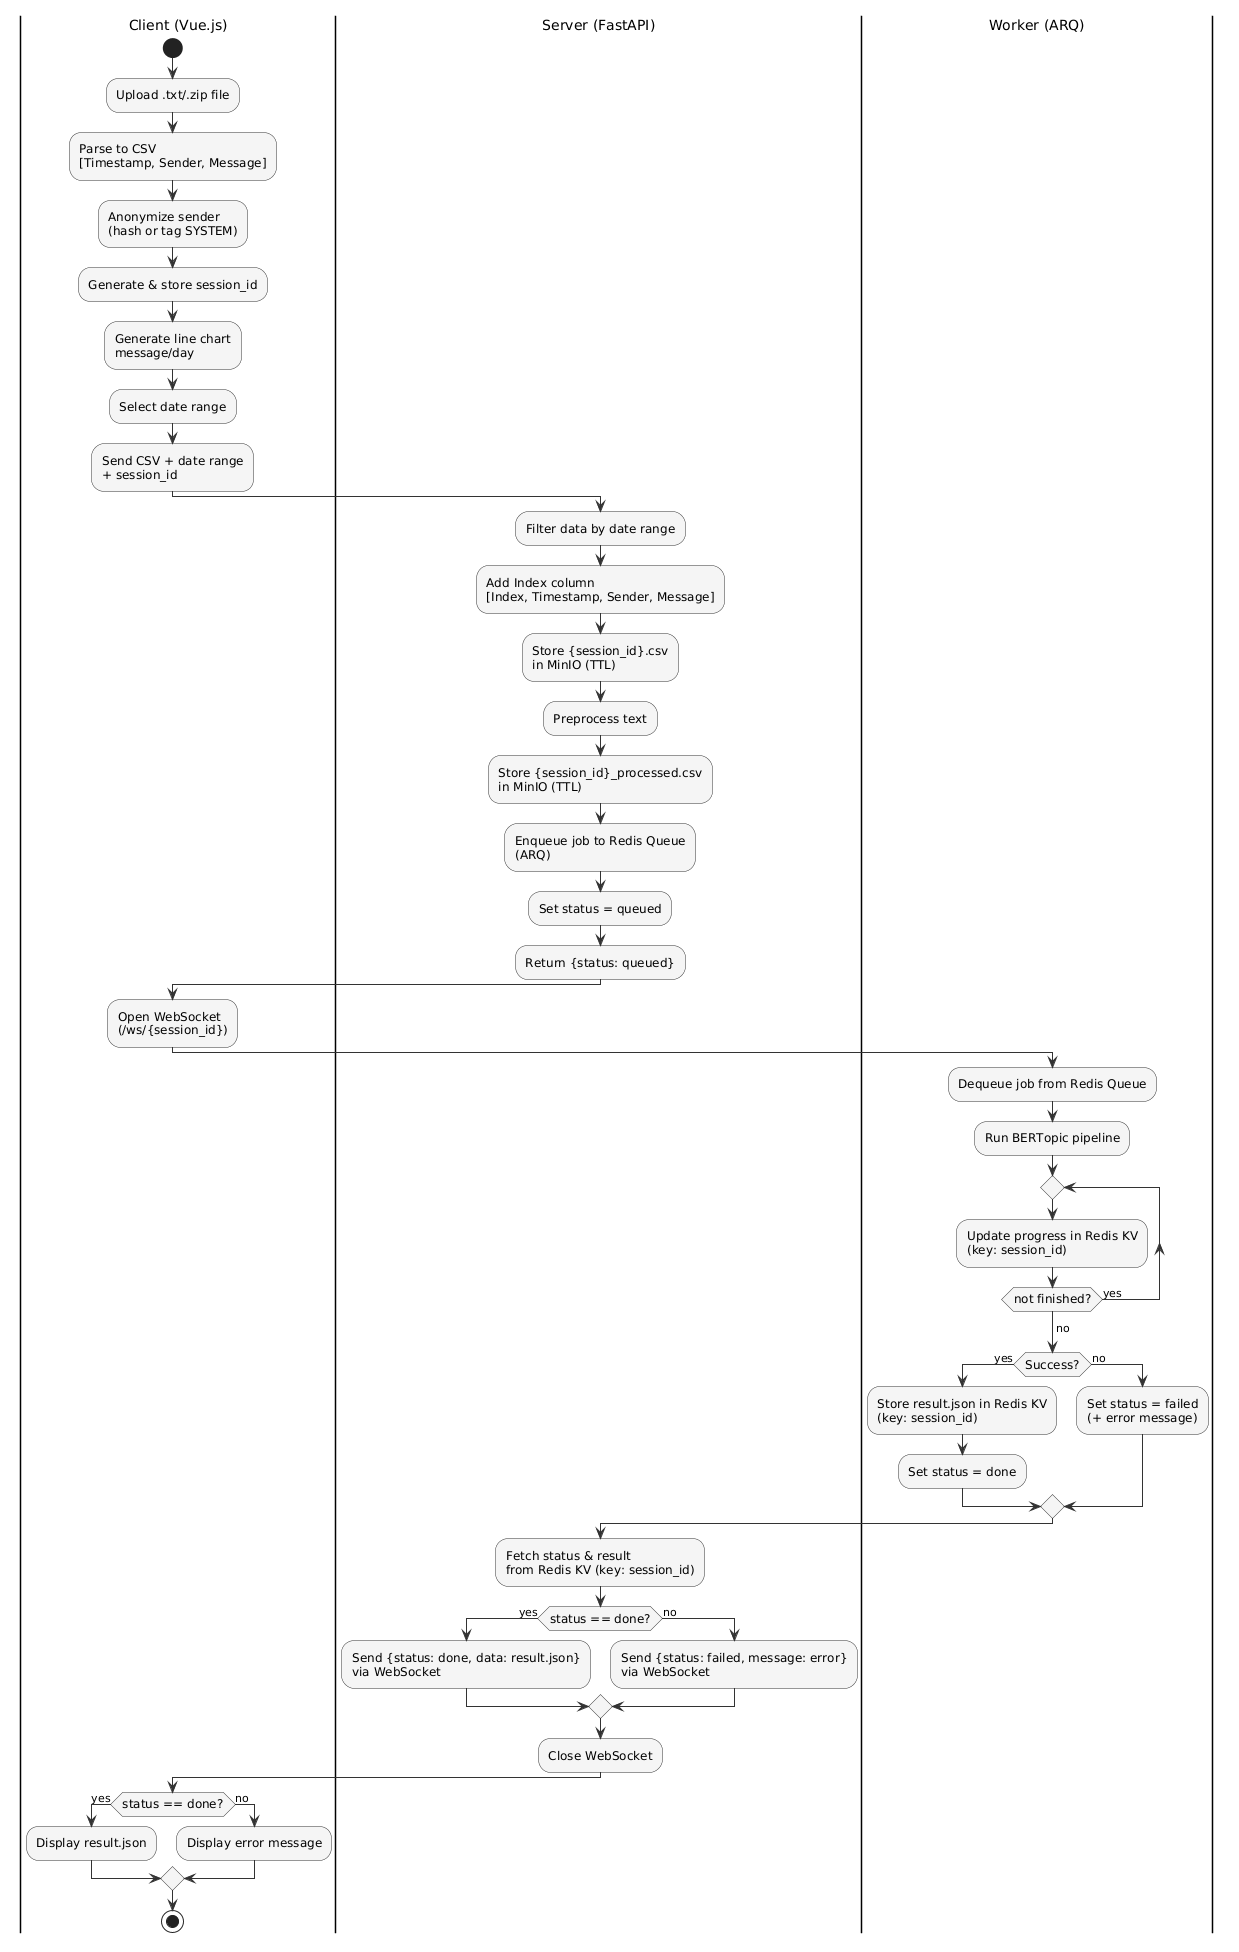
\includegraphics[width=0.9\textwidth]{images/bab-4-alur-teknis-implementasi-sistem.png}
\caption{Alur Teknis Implementasi Sistem}
\label{fig:bab-4-alur-teknis-implementasi-sistem}
\end{figure}


% ====================================================================
% CATATAN PENGISIAN LAMPIRAN:
%
% 1. JENIS LAMPIRAN YANG BIASA DISERTAKAN:
%    - Data mentah (raw data)
%    - Instrumen (kuesioner, interview guide, observation sheet)
%    - Output analisis (tabel detail, grafik dari software)
%    - Kode sumber (untuk komputasi/programming research)
%    - Dokumen administratif (surat izin, ICF, ethical clearance)
%    - Tabel/grafik pendukung yang terlalu besar untuk main text
%
% 2. ORGANISASI:
%    - Gunakan Lampiran A, B, C, dst. untuk kategorisasi
%    - Setiap lampiran harus direferensikan dalam main text
%    - Tambahkan deskripsi untuk clarity
%
% 3. FORMAT:
%    - Lampiran harus jelas dan mudah dibaca
%    - Gunakan numbering, labeling yang konsisten
%    - Sertakan captions dan figure/table references
%
% 4. UKURAN:
%    - Jangan membuat lampiran terlalu besar
%    - Untuk data besar, gunakan external file dan referensikan
%    - Dokumentasi external files dengan jelas
%
% 5. KEAMANAN DATA:
%    - Jangan masukkan data pribadi yang sensitif (nama, nomor identitas)
%    - Anonimisasi data jika diperlukan
%    - Pertimbangkan privasi responden
% ====================================================================
